% How to write a text along path using TikZ: Speedometer case
% https://latexdraw.com/
% 17/12/2019, 19:24

\documentclass[border=0.5cm]{standalone}

\usepackage{tikz}
\usetikzlibrary{decorations.text}

\begin{document}

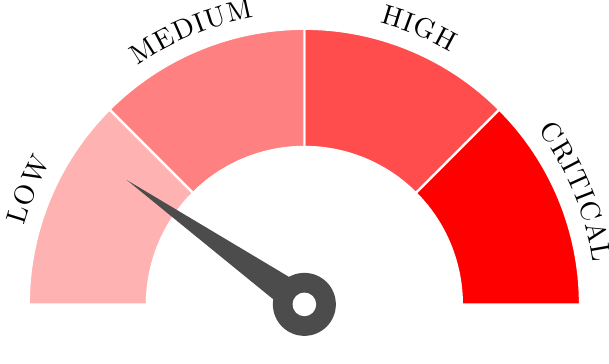
\begin{tikzpicture}[font=\small]
% Static part
\draw[draw=white,fill=red,thick] (0:2) -- (0:3.5) arc(0:45:3.5) -- (45:2) arc(45:0:2) -- cycle ;
\draw[draw=white,fill=red!70,thick] (90:2cm)-- (90:3.5cm) arc (90:45:3.5) -- (45:2cm) arc (45:90:2);
\draw[draw=white,fill=red!50,thick] (135:2cm)-- (135:3.5cm) arc (135:90:3.5) -- (90:2cm) arc (90:135:2);
\draw[draw=white,fill=red!30,thick] (135:2cm)-- (135:3.5cm) arc (135:180:3.5) -- (180:2cm) arc (180:135:2);


%Labels
\draw[decoration={text along path,
      text={LOW},text align={center},raise=0.2cm},decorate] (180:3.5cm) arc (180:135:3.5);

\draw[decoration={text along path,
      text={MEDIUM},text align={center},raise=0.2cm},decorate] (135:3.5cm) arc (135:90:3.5);

\draw[decoration={text along path,
      text={HIGH},text align={center},raise=0.2cm},decorate] (90:3.5cm) arc (90:45:3.5);

\draw[decoration={text along path,
      text={CRITICAL},text align={center},raise=0.2cm},decorate] (45:3.5cm) arc (45:0:3.5);


% Speedometer needle
\fill[black!70,rotate=145] (0,0.2)--(0:2.75) -- (0,-0.2)--cycle;
\fill [black!70](0,0) circle (0.4cm);
\fill [white](0,0) circle (0.15cm);

\end{tikzpicture}

\end{document}

% https://latexdraw.com/
% 17/12/2019, 19:24

\documentclass[border=0.5cm]{standalone}

\usepackage{tikz}
\usetikzlibrary{decorations.text}

\begin{document}

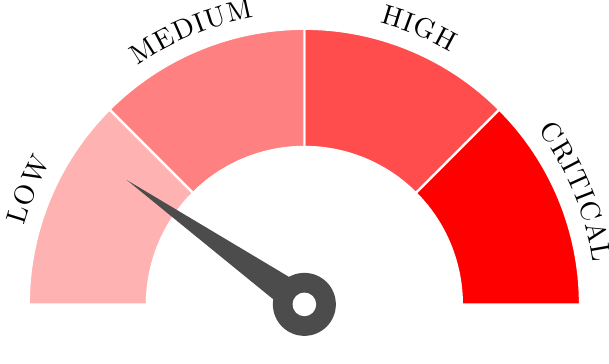
\begin{tikzpicture}[font=\small]
% Static part
\draw[draw=white,fill=red,thick] (0:2) -- (0:3.5) arc(0:45:3.5) -- (45:2) arc(45:0:2) -- cycle ;
\draw[draw=white,fill=red!70,thick] (90:2cm)-- (90:3.5cm) arc (90:45:3.5) -- (45:2cm) arc (45:90:2);
\draw[draw=white,fill=red!50,thick] (135:2cm)-- (135:3.5cm) arc (135:90:3.5) -- (90:2cm) arc (90:135:2);
\draw[draw=white,fill=red!30,thick] (135:2cm)-- (135:3.5cm) arc (135:180:3.5) -- (180:2cm) arc (180:135:2);


%Labels
\draw[decoration={text along path,
      text={LOW},text align={center},raise=0.2cm},decorate] (180:3.5cm) arc (180:135:3.5);

\draw[decoration={text along path,
      text={MEDIUM},text align={center},raise=0.2cm},decorate] (135:3.5cm) arc (135:90:3.5);

\draw[decoration={text along path,
      text={HIGH},text align={center},raise=0.2cm},decorate] (90:3.5cm) arc (90:45:3.5);

\draw[decoration={text along path,
      text={CRITICAL},text align={center},raise=0.2cm},decorate] (45:3.5cm) arc (45:0:3.5);


% Speedometer needle
\fill[black!70,rotate=145] (0,0.2)--(0:2.75) -- (0,-0.2)--cycle;
\fill [black!70](0,0) circle (0.4cm);
\fill [white](0,0) circle (0.15cm);

\end{tikzpicture}

\end{document}
